\documentclass[a4paper]{article}
\usepackage{amsmath,amssymb}
\usepackage[T2A]{fontenc}
\usepackage[russian]{babel}
\usepackage[utf8]{inputenc}
\usepackage{csquotes}
\usepackage{graphicx}
\usepackage{geometry}
\usepackage{enumitem}
\usepackage{mathtools}
\usepackage{float}
\usepackage{wrapfig}
\usepackage{amsmath}
\usepackage{siunitx}
\usepackage{enumitem}
\usepackage[utf8]{inputenc}
\usepackage{siunitx}
\usepackage{csquotes}
\usepackage[backend=biber, style=gost-numeric]{biblatex} % ГОСТ стиль
\addbibresource{ковальчук2017развитие.bib}
\addbibresource{сыромятников2022нейтронная.bib}

\title{Введение к рефлектометрии}
\author{}
\date{}

\begin{document}

\maketitle

\section{Классификация нейтронных источников}
Нейтронная рефлектометрия представляет собой мощный метод исследования поверхностей и многослойных структур, который позволяет получать детальную информацию о толщине, шероховатости и химическом составе слоев с разрешением на нанометровом уровне. Ключевым элементом любой нейтронной рефлектометрической установки выступает источник нейтронов, который определяет как возможности, так и ограничения данного метода.

Нейтронные источники классифицируются на два основных типа: стационарные и импульсные. Принципиальное различие между ними заключается в характере генерации нейтронного потока, что непосредственно влияет на конструкцию рефлектометров и применяемые методы монохроматизации. Эти особенности, в свою очередь, определяют параметры нейтронных потоков, что впоследствии оказывает существенное влияние на специфику и возможности проводимых экспериментов.

\section*{Создание нейтронных пучков для нейтронной рефлектометрии}

Для задач нейтронной рефлектометрии необходимо создать поток нейтронов с определённой энергией, поляризацией и направлением движения.

Источники нейтронов делятся на два типа: стационарные и импульсные.

Стационарные источники нейтронов характеризуются постоянным нейтронным потоком от контролируемой реакции ядерного деления в ядерном реакторе, могут базироваться на следующих реакциях:

\begin{itemize}
    \item Спонтанное деление ядер:
    \begin{align*}
        ^{252}\text{Cf} &\to \text{осколки деления} + \sim3.77\,\text{нейтрона/деление} + \sim\SI{200}{MeV} \\
        ^{240}\text{Pu} &\to \text{осколки деления} + \sim2.2\,\text{нейтрона/деление} + \sim\SI{200}{MeV}
    \end{align*}
    
    \item Радионуклидные ($\alpha$,n)-источники --- комбинация $\alpha$-излучателя (например, \(^{241}\text{Am}\), \(^{226}\text{Ra}\), \(^{210}\text{Po}\)) и мишени из легкого элемента (обычно Be, Li или B), при взаимодействии происходит реакция вида:
    \[
    \alpha + {}^9\text{Be} \to {}^{12}\text{C} + n
    \]
    
    \item Фотонейтронные источники --- $\gamma$-излучение взаимодействует с ядрами определенных элементов:
    \begin{align*}
        ^9\text{Be} + \gamma &\to {}^8\text{Be} + n + \SI{1.67}{MeV} \\
        ^2\text{H} + \gamma &\to {}^1\text{H} + n + \SI{2.22}{MeV}
    \end{align*}
    
    \item Ядерные реакторы --- поддерживаемая цепная реакция деления тяжелых ядер:
    \begin{align*}
        ^{235}\text{U} + n &\to \text{осколки деления} + \sim2.43\,\text{нейтрона/деление} + \sim\SI{200}{MeV} \\
        ^{239}\text{Pu} + n &\to \text{осколки деления} + \sim2.87\,\text{нейтрона/деление} + \sim\SI{200}{MeV}
    \end{align*}
\end{itemize}

Импульсные источники могут базироваться на:

\begin{itemize}
    \item Механическом прерывателе (чоппере) со стационарным источником. Непрерывный поток нейтронов прерывается вращающимся механическим устройством, поток «нарезается» на короткие импульсы с частотой вращения прерывателя.
    
    \item Ускоритель заряженных частиц в импульсном режиме с мишенью.
    
    \item Импульсные реакторы. Механизм генерации импульса:
    \begin{itemize}
        \item Реактор сначала приводится в подкритическое состояние,
        \item затем быстро вводится положительная реактивность (например, перемещением отражателя, извлечением поглотителя или специальными импульсными стержнями),
        \item мощность реактора начинает экспоненциально расти,
        \item рост прекращается за счет отрицательной обратной связи (тепловое расширение топлива, доплеровский эффект),
        \item после пика мощность быстро падает.
    \end{itemize}
    
    \item Создание условий для термоядерного синтеза:
    \begin{align*}
        ^2\text{H} + {}^3\text{H} &\to {}^4\text{He} + n + \SI{17.6}{MeV} \\
        ^2\text{H} + {}^2\text{H} &\to {}^3\text{He} + n + \SI{3.27}{MeV}
    \end{align*}
    Лазерный синтез: мощные лазерные импульсы сжимают мишень; \\
    Z-пинч устройства: сверхвысокий ток создает мощное магнитное поле.
\end{itemize}

Нейтронная рефлектометрия применяется для изучения твёрдых тел с характерным межатомарным расстоянием в кристаллической решётке около \SI{1}{\angstrom}. Для исследования таких структур требуется излучение с соответствующей длиной волны. Для нейтронов такая длина волны достигается при энергиях порядка 0.01 эВ, что соответствует холодным нейтронам. Однако первичный спектр нейтронов от ядерного реактора довольно широк, максимум спектральной плотности приходится на энергии порядка 2 МэВ, что явно не подходит для задач нейтронной рефлектометрии. Это энергетическое несоответствие требует создания специализированных систем для замедления нейтронов до требуемого энергетического диапазона.

\subsection*{Процесс замедления нейтронов}

Замедление нейтронов из реакторных источников включает несколько этапов:

\begin{enumerate}
    \item Начальное замедление с помощью бериллия непосредственно в активной зоне реактора
    
    \item Последующее замедление с использованием водных замедлителей (как H\textsubscript{2}O, так и D\textsubscript{2}O) для снижения энергии нейтронов до уровня, требуемого для экспериментов по рефлектометрии
    
    \item Транспортировка по нейтроноводам, которые также смещают пик энергетического спектра в область более низких энергий
\end{enumerate}

\begin{figure}[H]
    \centering
    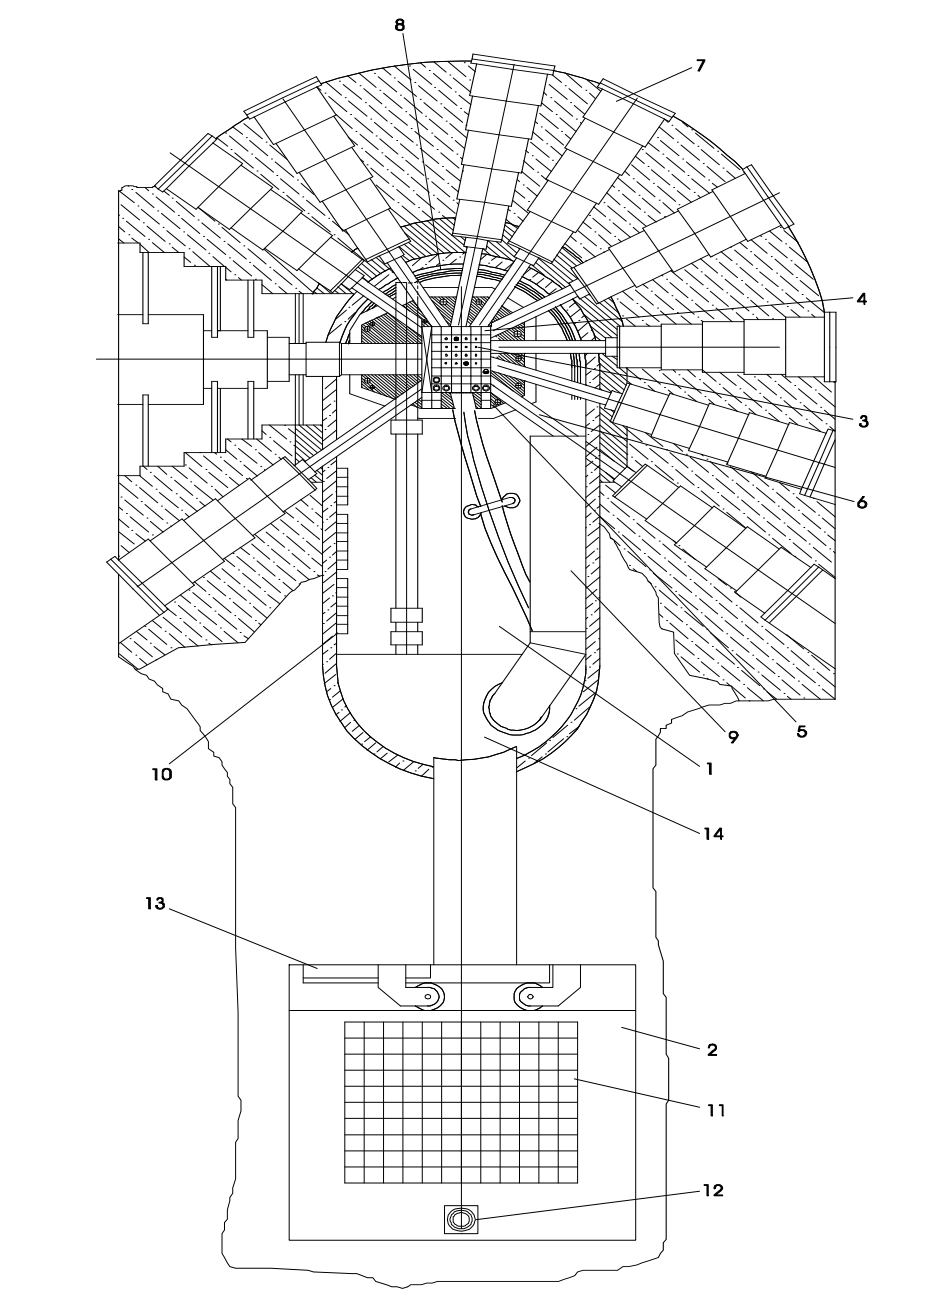
\includegraphics[width=0.73\textwidth]{разрез_ир8.png}
    \caption{Поперечный разрез реактора ИР-8: 
        1 – бассейн реактора; 
        2 – бассейн хранилища; 
        3 – ТВС; 
        4 – сменный бериллиевый блок; 
        5 – стационарный бериллиевый блок; 
        6 – Горизонтальный экспериментальный канал; 
        7 – шибер; 
        8 – стальной экран; 
        9 – задерживающая емкость; 
        10 – временное хранилище ОТВС; 
        11 – хранилище ОТВС; 
        12 – ведро контейнера для выгрузки ТВС из бассейна; 
        13 – ворота шлюза; 
        14 – крышка распределительного короба}
    \label{fig:ir8-cutaway}
\end{figure}

\subsection*{Транспортировка холодных нейтронов}

Холодные нейтроны доставляются к рефлектометрам по нейтроноводам. Эти нейтроноводы спроектированы с определенными оптическими свойствами для эффективной транспортировки нейтронов с сохранением желаемых характеристик пучка.

Типы нейтроноводов:

\begin{enumerate}
    \item Прямые --- базовая транспортировка с постоянным сечением
    
    \item Изогнутые --- устраняют прямую видимость источника, снижая фон излучения
    
    \item Баллистические --- с расширяющимися/сужающимися секциями для минимизации потерь
    
    \item Переменного сечения (эллиптические, параболические) --- оптимизируют характеристики пучка
    
    \item Фокусирующие --- концентрируют пучки для увеличения плотности потока
\end{enumerate}

Материалы:

\begin{itemize}
    \item Никель --- высокие критические углы
    
    \item Суперзеркальные покрытия (многослойные Ni/Ti)
    
    \item Подложки: борированное стекло, кремний, алюминий
\end{itemize}

Суперзеркала характеризуются $m$-значением --- отношением критического угла к углу природного никеля, что значительно повышает эффективность транспортировки.

\bigskip

Так, например, исследовательский ядерный реактор бассейнового типа ИР-8 (рис. 1, 2) предназначен для проведения фундаментальных и прикладных исследований в различных областях науки и техники: в области ядерной физики, физики твёрдого тела и сверхпроводимости, нанотехнологий и наноматериалов, радиационного материаловедения, нейтронно-активационного анализа элементного состава вещества, испытаний образцов новых топливных композиций для перспективных энергетических реакторных установок, наработки изотопов медицинского назначения. Активная зона реактора расположена под десятиметровым слоем дистиллированной воды, а в активной зоне используются бериллиевые блоки. На реакторе имеется 12 горизонтальных каналов, из которых:

\begin{itemize}
    \item 9 радиальных ГЭК с внутренним диаметром 100 мм;
    
    \item 1 касательный сквозной ГЭК с внутренним диаметром 150 мм;
    
    \item 1 специальный ГЭК с внутренним диаметром 230 мм, используемый для размещения в нем источника холодных нейтронов;
    
    \item 1 криволинейный ГЭК для вывода ультрахолодных нейтронов.
\end{itemize}

В настоящее время на ГЭК № 10 экспериментальные устройства и оборудование демонтированы. На этом канале сооружается источник холодных нейтронов с комплексом нейтроноводов и экспериментальных установок. Источник холодных нейтронов предназначен для формирования интенсивного потока нейтронов с длиной волны \(\sim\SI{4}{\angstrom}\).

Для проведения исследований на горизонтальных каналах реактора ИР-8 имеется комплекс нейтронно-физической аппаратуры, в состав которого входят различные исследовательские инструменты, в том числе:

\begin{itemize}
    \item Нейтронный рефрактометр;
    
    \item Трёхосный кристаллический спектрометр;
    
    \item Поликристалльный многодетекторный кольцевой дифрактометр;
    
    \item Трёхосный спектрометр на идеальных кристаллах.
\end{itemize}

\begin{figure}[h]
    \centering
    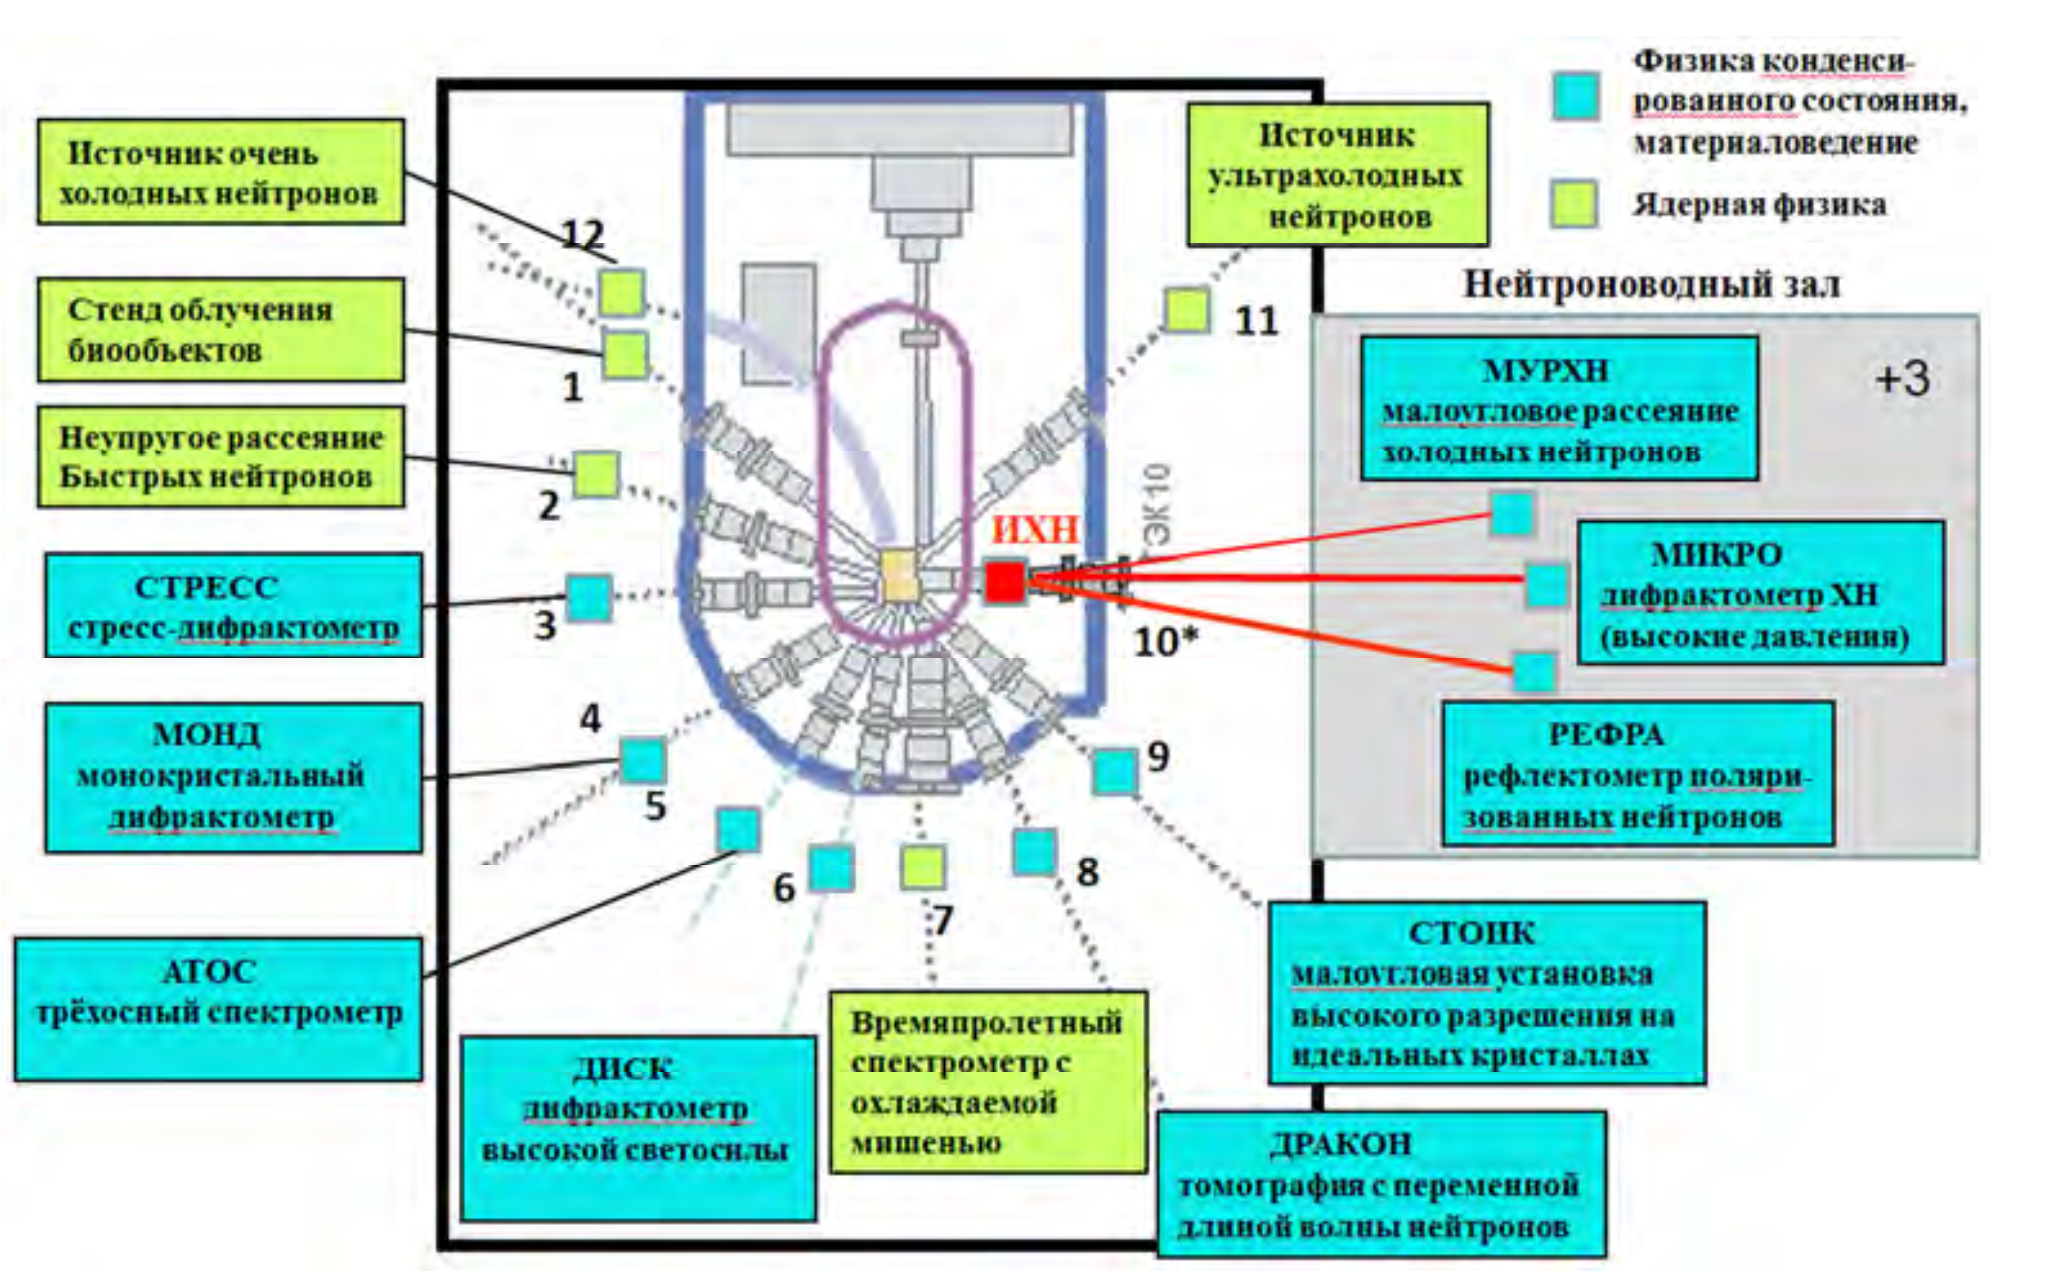
\includegraphics[width=0.8\textwidth]{ир8.png}
    \caption{ Курчатовский нейтронный центр на базе реактора ИР-8}
\end{figure}

Планируется установить три нейтроновода, 
на выходе которых интегральный поток нейтронов будет 
\(2 \times 10^{8}\,\text{\textit{см}}^{-2}\text{\textit{с}}^{-1}\) 
с максимумом спектра вблизи длины волны нейтронов \(4{,}5\,\text{\AA}\). 
На нейтроноводах будут установлены три установки: 
спектрометр малоуглового рассеяния холодных нейтронов (МУРХН), 
дифрактометр для исследования микрообразцов под высоким давлением (МИКРО) 
и рефлектометр поляризованных нейтронов (РЕФРА).
%\cite{ковальчук2017развитие}


\subsection{Стационарные источники нейтронов}
Стационарные источники, представленные преимущественно исследовательскими ядерными реакторами (ИР-8, ПИК, ИВВ-2М), производят непрерывный поток нейтронов с широким энергетическим спектром. Первичный спектр тепловых нейтронов описывается максвелловским распределением:

\begin{equation}
A(\lambda) \sim \lambda^{-5} \exp\left(-\frac{h^2}{2mk T\lambda^2}\right)
\end{equation}

где $h$ -- постоянная Планка, $m$ -- масса нейтрона, $k$ -- постоянная Больцмана, $T$ -- температура замедлителя.

При термализации нейтронов в активной зоне реактора максимум спектральной плотности приходится на длину волны $\lambda_{max} = \sqrt{\frac{5h^2}{2mkT}}$. Для реактора с температурой замедлителя $T = 300$ К оптимальная длина волны составляет около 1.45 \AA, что соответствует энергии нейтронов примерно 39 мэВ.

На стационарных источниках монохроматизация нейтронного пучка осуществляется с помощью кристаллических монохроматоров, использующих брэгговское отражение:

\begin{equation}
\lambda = 2d \cdot \sin(\theta_M)
\end{equation}

где $d$ -- межплоскостное расстояние в кристалле, $\theta_M$ -- угол скольжения.

Пучок, отраженный от монохроматора, имеет расходимость, 
которая определяется сверткой расходимости падающего пучка $\Delta\theta_{in}$ и мозаичности кристалла $\eta$:

\begin{equation}
\frac{1}{(\Delta\theta_{out})^2} = \frac{1}{(\Delta\theta_{in})^2} + \frac{1}{\eta^2}
\end{equation}

При этом относительная монохроматичность пучка связана с расходимостью соотношением:

\begin{equation}
\frac{\Delta\lambda}{\lambda} = \Delta\theta \cdot \cot(\theta_M)
\end{equation}

В данном случае аппаратная функция рефлектометра характеризуется разрешением по переданному импульсу:

\begin{equation}
\frac{\Delta q}{q} = \sqrt{\left(\frac{\Delta\theta}{\theta}\right)^2 + \left(\frac{\Delta\lambda}{\lambda}\right)^2}
\end{equation}

Оптимизация светосилы рефлектометра на стационарном источнике достигается при соотношении:

\begin{equation}
\frac{\Delta\theta}{\theta} = \frac{1}{2} \cdot \frac{\Delta q}{q}
\end{equation}

что позволяет максимизировать интенсивность при заданном разрешении.

\subsection{Импульсные источники нейтронов}
Импульсные источники включают:
\begin{itemize}
    \item Ускорители с мишенями (ISIS, SNS, ESS), использующие реакции скалывания при бомбардировке тяжелых мишеней высокоэнергетическими частицами 
    \item Импульсные реакторы (ИБР-2) 
    \item Лазерные нейтронные источники, основанные на DD- или DT-реакциях синтеза 
\end{itemize}

В таких системах нейтроны генерируются короткими импульсами, что позволяет применять времяпролетный метод (TOF) для определения длины волны нейтронов:

\begin{equation}
\lambda = \frac{h \cdot t}{m \cdot L}
\end{equation}

где $t$ -- время пролета, $L$ -- расстояние от источника до детектора.

Времяпролетная методика позволяет измерять кривые отражения в широком диапазоне длин волн за один импульс источника, что существенно увеличивает эффективность использования нейтронного потока. Основное разрешение в этом случае определяется временным разрешением:

\begin{equation}
\frac{\Delta\lambda}{\lambda} = \frac{\Delta t}{t}
\end{equation}

В зависимости от типа прерывателя (чоппера) в системе, аппаратная функция может быть разной:
\begin{enumerate}
    \item Однодисковый прерыватель обеспечивает постоянное времяпролетное разрешение $\Delta t$, поэтому $\Delta\lambda = \text{const}$, что приводит к $\frac{\Delta\lambda}{\lambda} \sim \frac{1}{\lambda}$. 
    \item Двухдисковый прерыватель позволяет получить $\frac{\Delta\lambda}{\lambda} = \text{const}$ во всем диапазоне длин волн. 
\end{enumerate}

При времяпролетной методике разрешение по переданному импульсу выражается как:

\begin{equation}
\frac{\Delta q}{q} = \sqrt{\left(\frac{\Delta\theta}{\theta}\right)^2 + \left(\frac{\Delta t}{t}\right)^2}
\end{equation}

Оптимизация светосилы рефлектометра на импульсном источнике достигается при условии:

\begin{equation}
\frac{\Delta\theta}{\theta} = \frac{1}{\sqrt{2}} \cdot \frac{\Delta t}{t}
\end{equation}

\subsection{Влияние температуры источника}
Существенным фактором является температура нейтронного источника. Для тепловых источников ($T \approx 300$ К) максимум спектра приходится на $\lambda \approx 1.12$ \AA, для холодных ($T \approx 30$ К) -- на $\lambda \approx 3.56$ \AA. При прочих равных условиях, переход к холодному источнику увеличивает светосилу рефлектометра пропорционально $\sqrt{\frac{T_1}{T_2}}$, что для указанных температур дает прирост примерно в 3.16 раза.

Холодные нейтроны также обеспечивают лучшее $q$-разрешение, поскольку при той же коллимации пучка $\Delta\theta$ относительная монохроматичность $\frac{\Delta\lambda}{\lambda}$ улучшается с ростом длины волны $\lambda$. Кроме того, эффективность транспортировки нейтронов от источника к образцу выше для холодных нейтронов из-за более эффективного захвата и удержания их в нейтроноводах.

Таким образом, выбор типа нейтронного источника и его характеристик определяет подход к монохроматизации нейтронного пучка, конструкцию рефлектометра и, в конечном счете, аппаратную функцию прибора, что напрямую влияет на возможности и ограничения экспериментальных исследований.

\section{Свёртка. Аппаратная функция}

Свёртка – операция, применяющаяся к двум функциям, возвращающая их взаимнокорреляционную функцию. Так, применяя оператор
свёртки для истинного распределения и аппаратной функции, получим измеренное распределение физической величины. 

\begin{figure}[h]
    \centering
    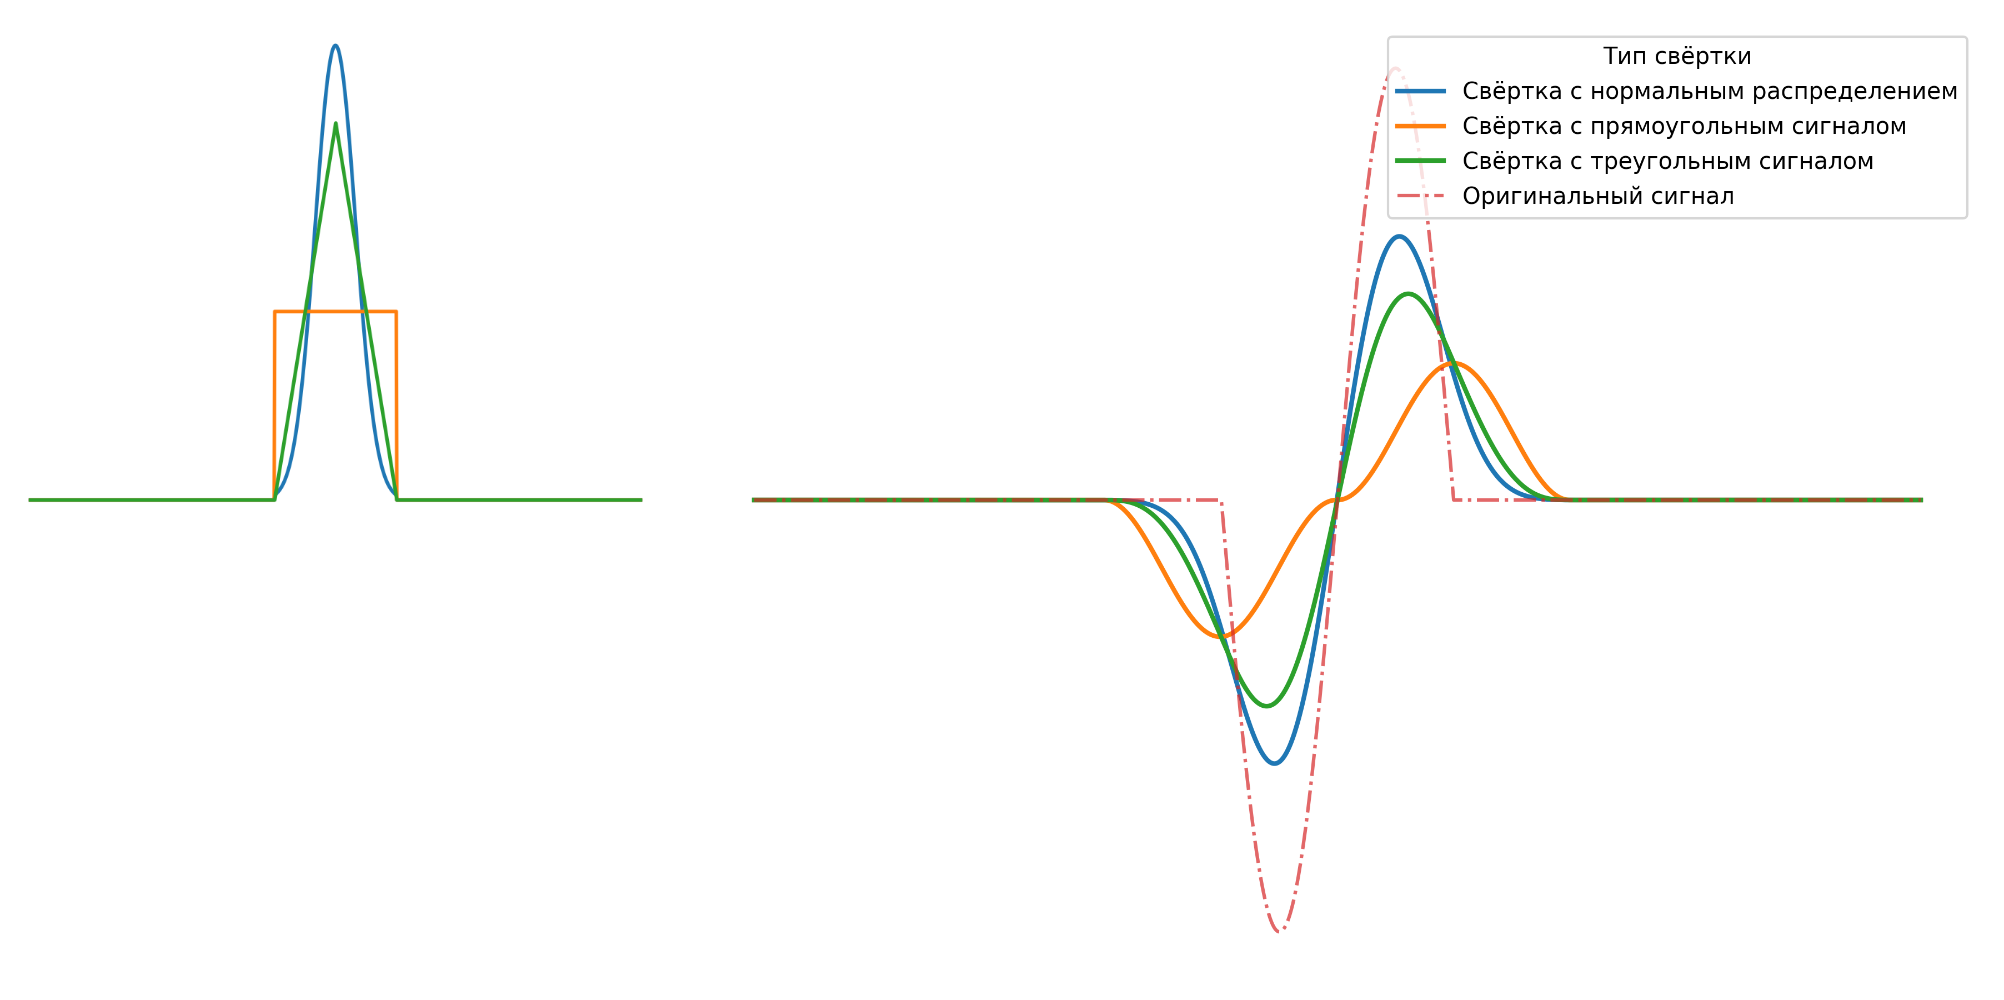
\includegraphics[width=0.7\textwidth]{conv_h.png}
    \caption{Иллюстрация работы свёртки}
\end{figure}

Свёртка играет важную роль в моделировании искажений, связанных с ограниченным разрешением измерительных устройств.
Поскольку приборы не способны идеально воспроизводить входной сигнал (например, из-за физических ограничений оптики или
электроники), их влияние на измеряемую величину можно описать как свёртку истинного распределения $\varphi
\left(x\right)$ с аппаратной функцией $a\left(x\right)$. Это позволяет теоретически предсказать, как будут выглядеть
экспериментальные данные при заданных параметрах установки.

На практике задача восстановления исходного распределения $\varphi \left(x\right)$ из измеренного сигнала 
$f\left(x\right)$ (т.н. обратная свёртка) является сложной и решается лишь в специальных случаях, например, при
определённых условиях гладкости функций или наличии априорной информации о системе. Наиболее часто свёртка используется
для симуляции ожидаемых искажений. Например, при проектировании спектрометров или радиотелескопов с её помощью
моделируют ``размытие'' спектральных линий или изображений, что помогает оценить пределы
разрешающей способности прибора и скорректировать экспериментальные параметры.

\textbf{Теорема о свёртке.}

Если $h(x) = (f \ast g)(x)$ --- свёртка функций $f(x)$ и $g(x)$, то их преобразования Фурье удовлетворяют соотношению:

\begin{equation}
\mathcal{F}\{h\}(k) = \mathcal{F}\{f\}(k) \cdot \mathcal{F}\{g\}(k)
\end{equation}

где:
\begin{itemize}
\item $\mathcal{F}\{f\}(k) = \int_{-\infty}^{+\infty} f(x)e^{-ikx}dx$ --- преобразование Фурье функции $f(x)$
\item $\mathcal{F}\{g\}(k)$ --- преобразование Фурье функции $g(x)$
\end{itemize}

\textbf{Обратное преобразование.}

Свёртка в исходном пространстве восстанавливается через обратное преобразование Фурье:

\begin{equation}
h(x) = \mathcal{F}^{-1}\{\mathcal{F}\{f\} \cdot \mathcal{F}\{g\}\}
\end{equation}

В исследованиях возникают как задачи, связанные с вычислением истинного распределения $\varphi \left(x\right)$, так и
задачи, связанные с моделированием измеренного распределения $f\left(x\right)$ физической величины с учётом параметров
установки.

Задача нахождения $\varphi \left(x\right)$ сводится к решению интегрального уравнения (1) с помощью преобразования
Фурье, при этом решение может быть выполнено только для некоторых видов функций $f\left(x\right)$ и 
$a\left(x\right)$.

\textbf{Аппаратная функция.}

Аппаратная функция --- характеристика линейного измерительного устройства, устанавливающая связь измеренной величины на выходе устройства с истинным значением этой величины на его входе. Математически аппаратная функция определяется из уравнения

\begin{equation}
f(x) = \int_{-\infty}^{+\infty} a(x-x_1)\varphi(x_1)dx_1
\end{equation}

где $f(x)$ --- измеренное распределение физической величины, $\varphi(x)$ --- истинное распределение, $a(x)$ --- аппаратная функция.

Аппаратная функция может быть рассчитана теоретически по известным параметрам измерительного устройства, однако это
представляет собой достаточно сложную задачу и даёт, как правило, приближённые результаты. Поэтому очень часто
аппаратную функцию определяют экспериментальным путём. Так, аппаратная функция оптического спектрометра может быть
измерена с достаточно большой точностью, если для освещения входной щели использовать излучение с выхода другого
спектрометра с известной аппаратной функцией, на 1-2 порядка меньшей ширины, чем у данного, либо использовать источник
с узкой спектральной линией, в окрестностях которой перестраивается (по длинам волн, частотам или обратным сантиметрам)
спектрометр с измеряемой аппаратной функцией. При таком измерении форма и ширина аппаратной функции будут определены
точнее, чем расчётным путём, так как при этом учитываются даже неточности юстировки, которые никак не могут быть учтены
при расчёте. Рассчитанная или измеренная аппаратная функция реальных приборов на практике аппроксимируется с помощью
ряда функций.

Так, аппаратная функция является не только и не столько критерием разрешения, сколько характеристикой прибора, знание
которой позволяет вычислить истинное распределение в спектре величины, характеризующей изучаемое
явление. 

\section{Метод рефлектометрии}
Нейтронная рефлектометрия представляет собой мощный экспериментальный метод для исследования структуры поверхностей, тонких плёнок и многослойных систем на наномасштабе. В основе метода лежит физическое явление зеркального отражения нейтронов от плоских границ раздела сред при скользящих углах падения.
Уникальность нейтронов как зондирующих частиц обусловлена комплексом их физических свойств. \\

\begin{figure}[H]
    \centering
    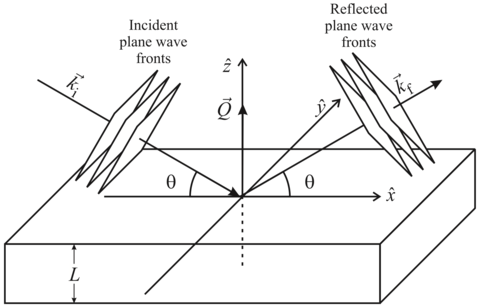
\includegraphics[width=0.7\textwidth]{refl_scheme.png}
    \caption{Отражение нейтронов от поверхности образца}
\end{figure}

Во-первых, электрическая нейтральность позволяет нейтронам беспрепятственно преодолевать кулоновский барьер и напрямую взаимодействовать с ядрами атомов. Это обеспечивает значительную глубину проникновения нейтронов в исследуемые материалы — до нескольких сотен нанометров, что существенно превосходит возможности многих поверхностно-чувствительных методов. \\
Во-вторых, длина волны тепловых нейтронов (\lambda = 0.1-10 $Å)   сопоставима с межатомными расстояниями в конденсированном веществе, что делает их идеальным инструментом для изучения атомной структуры материалов. При этом энергия тепловых нейтронов (5-100 мэВ) сравнима с энергией многих коллективных возбуждений в твердых телах. \\
В-третьих, взаимодействие нейтронов происходит непосредственно с атомными ядрами, а не с электронными оболочками, как в случае рентгеновского излучения. Это приводит к существенно иной зависимости сечения рассеяния от атомного номера элемента. Например, нейтроны весьма чувствительны к лёгким элементам, которые практически "прозрачны" для рентгеновских лучей. Более того, нейтроны способны различать изотопы одного элемента, что открывает широкие возможности для изотопного контрастирования в исследованиях сложных систем.
Наконец, нейтроны обладают собственным магнитным моментом, благодаря чему они чувствительны к магнитной микроструктуре исследуемых образцов. Это свойство позволяет методам нейтронного рассеяния получать уникальную информацию о магнитном упорядочении в веществе, что особенно ценно при изучении магнитных многослойных наноструктур, спиновых волн и магнитных доменов.
\\
Существуют два основных экспериментальных подхода к проведению измерений в нейтронной рефлектометрии, каждый из которых имеет свои преимущества и области применения - угловой и времяпролётный. \\
При использовании углового метода эксперимент проводится с монохроматическим пучком нейтронов с фиксированной длиной волны \lambda. $ Измерения коэффициента отражения R осуществляются путём последовательного изменения угла падения \theta $нейтронного пучка на поверхность образца. Переданный импульс в направлении нормали к поверхности при этом рассчитывается как:

\begin{equation}
 q_z=\frac{4\pi }{\lambda }\sin \theta,
\end{equation}
где $\lambda$ — длина волны нейтронов.\\
Преимущества данного метода включают высокое угловое разрешение и относительную простоту экспериментальной реализации. Угловой метод особенно эффективен на стационарных источниках нейтронов.
Типичный диапазон измерений углов составляет от 0° до 5-10°.\\
Альтернативным подходом является времяпролётная методика, которая особенно эффективна на импульсных источниках нейтронов. В этом случае угол падения \theta $ фиксируется, а измерения проводятся одновременно для нейтронов различных энергий и, соответственно, длин волн. Распределение нейтронов по энергиям определяется путём измерения времени их пролёта от источника до детектора.
Переданный импульс при этом меняется за счёт вариации длины волны $ \lambda $, где $\lambda$ зависит от времени пролёта t согласно соотношению (7).
Ключевые преимущества времяпролётного метода:
одновременное измерение в широком диапазоне $q_z$, 
отсутствие подвижных частей во время измерения,
высокая эффективность использования нейтронного пучка,
возможность работы с малыми образцами или слабыми сигналами.
Современные времяпролётные рефлектометры часто оснащаются позиционно-чувствительными детекторами, что позволяет одновременно регистрировать как зеркально отражённые нейтроны, так и диффузное рассеяние, несущее информацию о латеральных неоднородностях и шероховатости поверхности.\\

\bigskip

\section*{Постановка задачи}
Центральной задачей при анализе данных нейтронной рефлектометрии является восстановление профиля плотности длины рассеяния \rho(z)$ по измеренной зависимости коэффициента отражения R(q_z).$ Математически это представляет собой обратную задачу рассеяния, которая, в общем случае, не имеет однозначного решения.

\subsection*{1. Решение уравнения Шредингера для многослойных систем}
Разработка численного алгоритма расчёта коэффициента отражения нейтронов от вектора переноса импульса нейтронов в направлении, перпендикулярном поверхности образца с учётом:\\
•	послойного описания структуры мишени через распределение длины рассеяния;\\
•	шероховатости границ между слоями, задаваемой функцией ошибок;\\
•	векторизации вычислений для ускорения расчётов.

\subsection*{2. Оптимизация параметров структуры}
Разработка алгоритма подбора параметров структуры образца (толщин слоев, параметров шероховатости границ) в рамках заданных физических ограничений с целью минимизации расхождения между теоретической и экспериментальной кривыми нейтронной рефлектометрии. Алгоритм должен включать в себя:\\
•	модуль решения прямой задачи для расчета теоретической кривой отражения по текущим значениям параметров структуры;\\
•	оптимизационную процедуру, эффективно исследующую пространство параметров в поисках глобального минимума функции несоответствия.

\subsection*{3. Прогнозирование оптимальных измерений}
Разработать алгоритм динамического прогнозирования для определения последовательности измерений, максимизирующих информативность данных в реальном времени. Алгоритм должен:\\
•	использовать марковские цепи Монте-Карло (MCMC) для байесовского вывода апостериорных распределений параметров структуры и адаптивного обновления модели;\\
•	минимизировать информационную энтропию ключевых параметров через выбор точек, обеспечивающих максимальный ожидаемый прирост информации (Expected Information Gain);\\
•	учитывать физические ограничения эксперимента (время измерений, перемещение между точками, уровень шума) при планировании шагов;\\
•	автоматически останавливать измерения при достижении заданных критериев точности (порог энтропии, погрешность параметров);\\
•	интегрироваться с модулями численного решения и анализа для реализации замкнутого цикла: измерение → обновление модели → прогноз следующей точки.




\section*{Результаты}

В рамках исследования проведено численное моделирование работы экспериментального стенда для нейтронной рефлектометрии.
Основная цель моделирования — воспроизведение процессов взаимодействия нейтронов с тонкопленочными
структурами и получение зависимости коэффициента отражения от изменения волнового
вектора q\textsubscript{z}.

\bigskip

\subsection*{Стенд нейтронной рефлектометрии}

\begin{figure}[H]
\centering
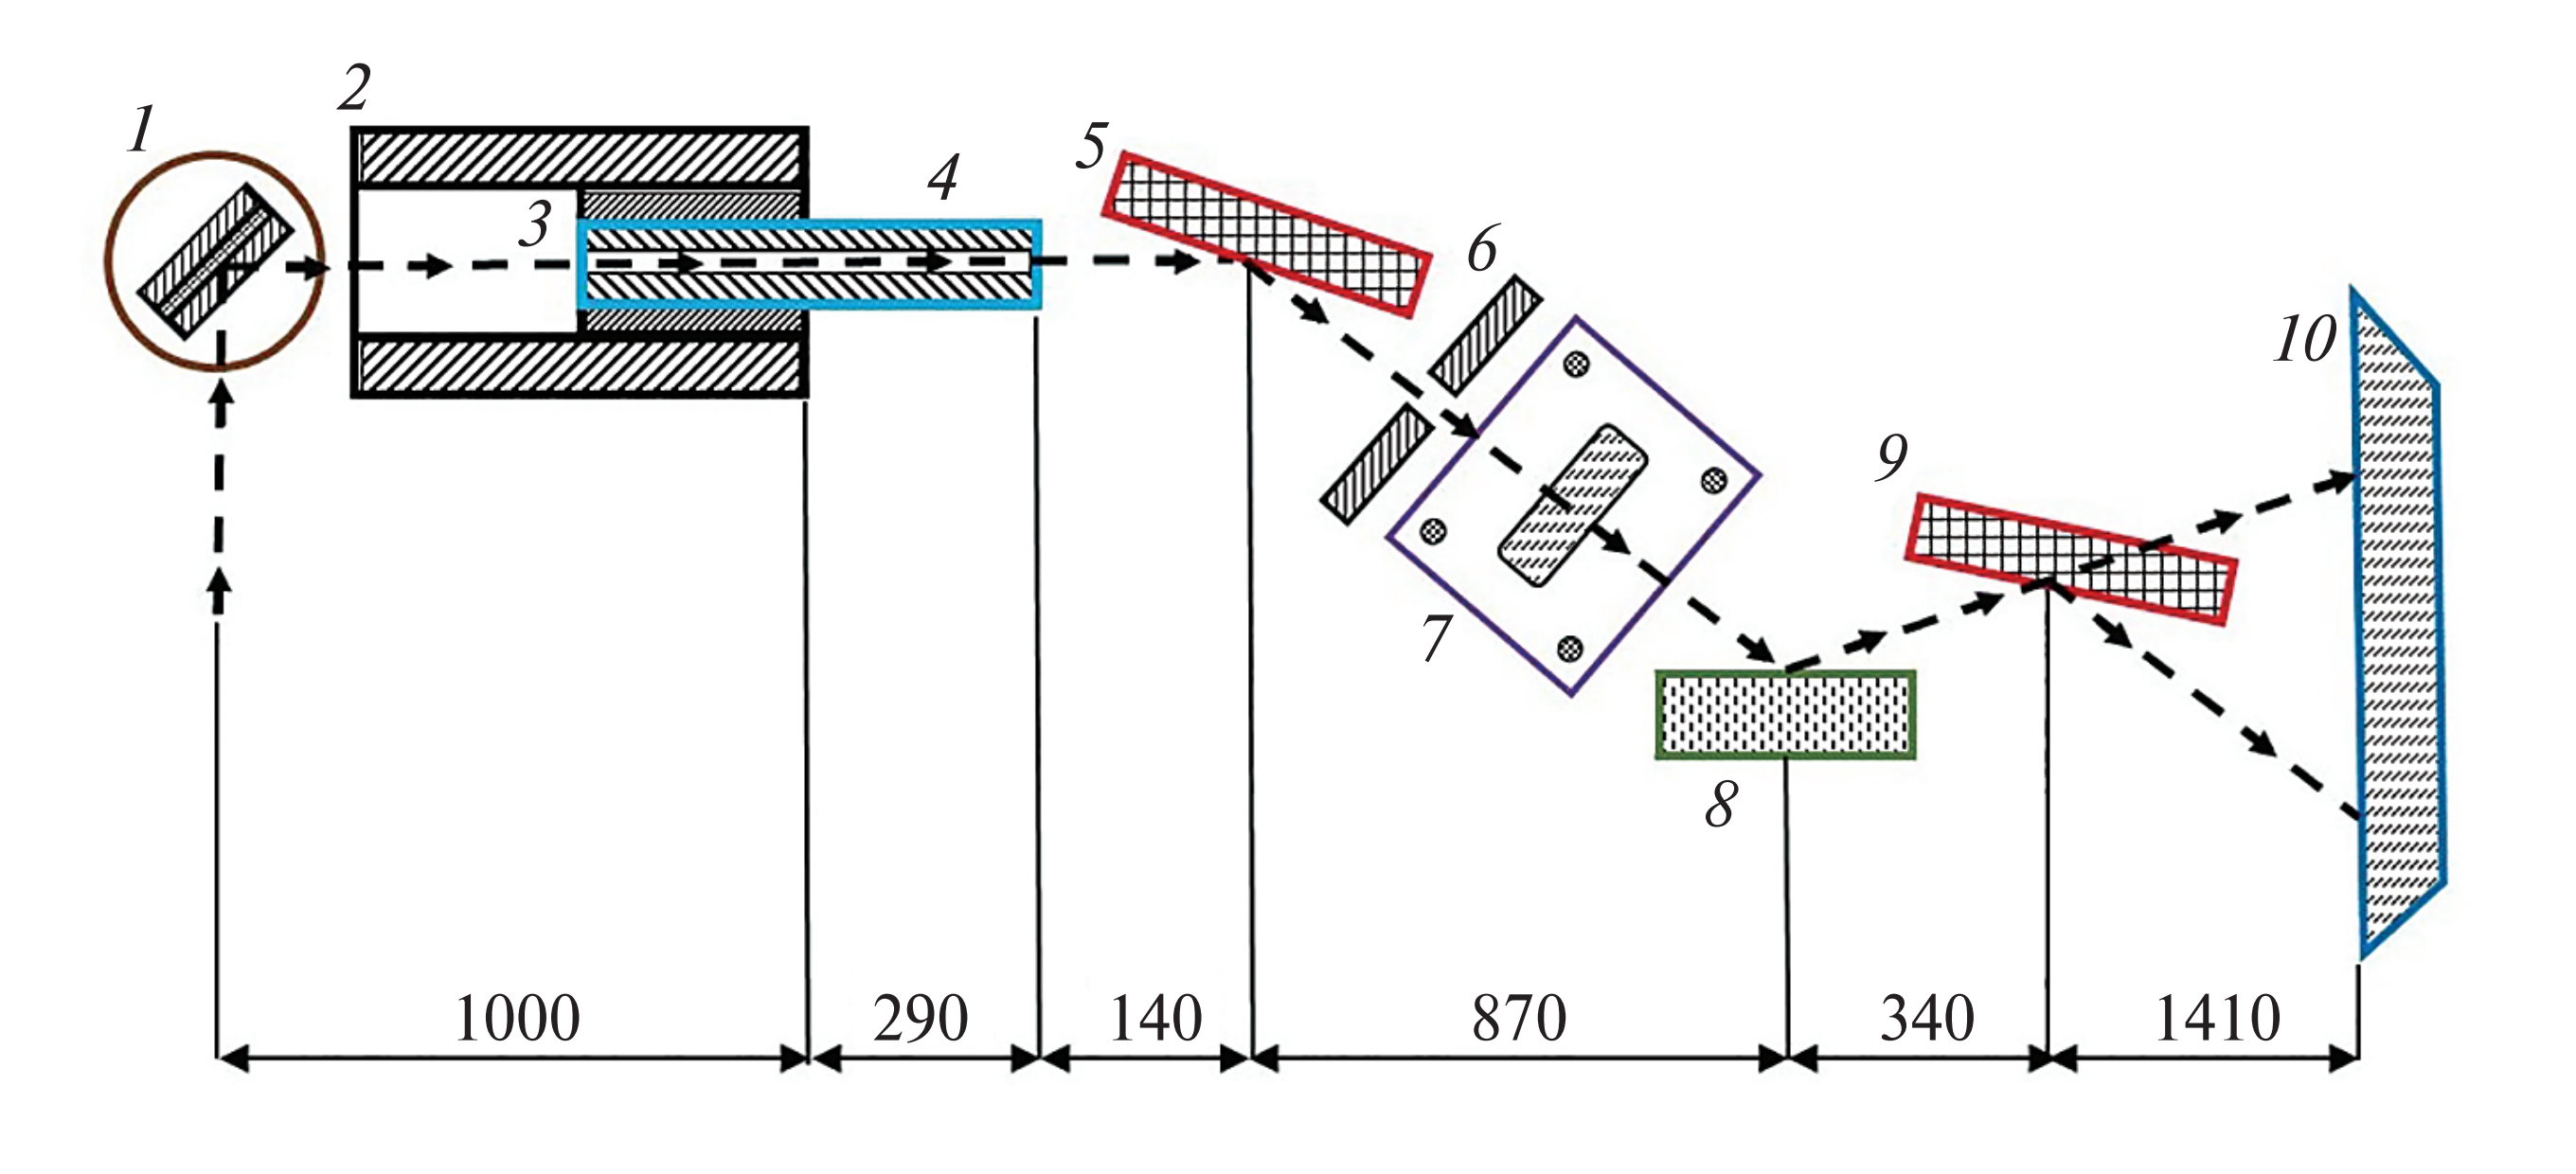
\includegraphics[scale=0.109]{a0000-img001.png}
\caption{Схема стенда нейтронной рефлектометрии: 1 — монохроматор Cu(111); 2 — ГЭК-5; 3 — коллиматор ГЭК5; 4 — вставка в коллиматор; 5 — суперзеркало-поляризатор; 6 — регулируемая щель; 7 — спин-флиппер; 8 — узел образца; 9 — суперзеркало-анализатор; 10 — одномерный позиционно-чувствительный детектор.}
\end{figure}


\bigskip

\section*{Решение прямой задачи рефлектометрии}

\begin{enumerate}
\item \textbf{Численное моделирование прямой задачи :}

Для решения задачи использован матричный метод, адаптированный для многослойных систем. В отличие от эксперимента, в модели не учитывается спиновая поляризация нейтронов, что упрощает расчёты, но сохраняет физическую достоверность для немагнитных материалов. Все матричные операции векторизованы для оптимизации вычислительных процессов, что позволяет сократить время расчётов без потери точности.

Решение задачи рефлектометрии базируется на решении классической задачи квантовой механики о прохождении волной потенциального барьера, где в роли волны выступают нейтроны, а в роли потенциального барьера  - образец. Математически, задача сводится к решению стационарного уравнения Шрёдингера:
\begin{align}
    \Bigg(\frac{\hbar^2}{2m_n}\nabla^2 + U(\vec{r})\Bigg)\Psi(\vec{r}) = E\Psi(\vec{r})
\end{align}
где m_n - $масса нейтрона, U(r) - потенциальная энергия

Заменив \begin{align}
\Psi(\vec{r}) = \psi(y)e^{{i} k_{||} q_{||}}
\end{align}

где \( k_{\parallel} \) - волновой вектор, параллельный поверхности образца,

и \(\psi(y)\) соответствует одномерному уравнению Шрёдингера:
\begin{equation}
    \left( \frac{d^2}{dy^2} + \left( \frac{2m_n}{\hbar^2}(E - U) - k_{\parallel}^2 \right) \right) \psi(y) = 0
\end{equation}

\text{Следовательно, для \alpha} \text {-го слоя имеем:}

\begin{equation}
    \Bigg( \frac{d^2}{dy^2} + q_{\alpha}^2 \Bigg) \psi(y) = 0
\end{equation}
где   q_{\alpha} = \Bigg(\frac{2m_n}{\hbar^2}(E - \frac{\hbar^2 k_{\parallel}^2}{2m_n} - U_{\alpha}) \Bigg)

Теперь можем записать волновую функцию в слое \alpha $как суперпозицию волн, 
распространяющихся по оси y и против оси y:

\begin{equation}
    \psi_{\alpha}(y) = a_{\alpha}e^{iq_{\alpha}(y- y_{\alpha})} + b_{\alpha}e^{-iq_{\alpha}(y- y_{\alpha})}
\end{equation}

Представим \psi_{\alpha}(y)|_{y = y_{\alpha}} $вектором \(
\begin{bmatrix}
a_{\alpha}\\
b_{\alpha}
\end{bmatrix}
\).

\text{Так, первой поверхности будет соответствовать:}
\psi_1 |_{y_1 = 0} = \(
\begin{bmatrix}
1\\
r
\end{bmatrix}
\) 

\text{Последней поверхности: } \psi_{n-1} |_{y_{n-1}} = \(
\begin{bmatrix}
t\\
0
\end{bmatrix} 
\) 

Следовательно, коэффициенты поглощения t и отражения r могут быть определены матрицой передачи:
\begin{equation}
     \(
\begin{bmatrix}
1\\
r
\end{bmatrix}
\)  = \(
\begin{bmatrix}
M_{11} & M_{12}\\
M_{21} & M_{22}
\end{bmatrix}
\) \(
\begin{bmatrix}
t\\
0
\end{bmatrix} 
\),
\end{equation}
 коэффициенты r и t могут быть выражены: 
\begin{equation}
    t = \frac{1}{M_{11}},  r = \frac{M_{21}}{M_{22}}
\end{equation}

Матрица передачи M выражается следующим образом:
\begin{equation}
    M = D^{-1}(q_1)\Bigg(\prod\limits_{j=2}^{N-1}[D(q_j)P(d_j , q_j)D^{-1}(q_j)]\Bigg)D(q_N),
\end{equation} \text{где} D(q_{\alpha}) - \text{матрица передачи, отвечающая за изменение абсолютного значения} \\
\text{волнового вектора в среде }  \alpha;

P(d_{\alpha} , q_{\alpha}) - \text{матрица распространения, отвечающая за изменение фазы волнового вектора}\\
\text{в среде } \alpha.

\begin{equation}
    D(q_{\alpha}) = \(
\begin{bmatrix}
1 & 1\\
q_{\alpha} & -q_{\alpha}
\end{bmatrix}
\)
\end{equation}

\begin{equation}
    P(q_{\alpha}, d_{\alpha}) = \(
\begin{bmatrix}
e^{-iq_{\alpha}d_{\alpha}} & 0\\
0 & e^{iq_{\alpha}d_{\alpha}}
\end{bmatrix}
\)
\end{equation}

Так, при использовании формул (21), (22), (23), (24), численно считается как модуль, так и фаза коэффициента отражения нейтронов от образца, при заданных параметрах его структуры.
Наибольшую трудоёмкость с точки счёта вызывает вычисление матрицы передачи (22). Вычисления кратно ускорены, так как векторизованы, что позволяет переложить их на ядра CUDA, или задействовать векторные инструкции процессора. 

\item \textbf{Учет конечного разрешения установки:}

Для приближения численных результатов к экспериментальным данным в модель введена аппаратная функция, описывающая искажения, связанные с техническими характеристиками стенда:

\begin{equation}
\Delta q = \frac{4\pi}{\lambda} \sqrt{(\Delta\theta)^2 + \theta^2\left(\frac{\Delta\lambda}{\lambda}\right)^2}
\end{equation}

\begin{itemize}
\item Угловое разрешение $\Delta\theta$, обусловленное коллимацией, можно варьировать
\item Разрешение по длине волны $\frac{\Delta\lambda}{\lambda} \approx 1\%$, задано монохроматором
\end{itemize}

Аппаратная функция представлена гауссовым профилем $G(q_z)$. Теоретическая зависимость $R_{\text{теор}}(q_z)$ преобразована в «экспериментальную» $R_{\text{эксп}}(q_z)$ через операцию свёртки:

\begin{equation}
R_{\text{эксп}}(q_z) = \int\limits_{-\infty}^{\infty} R_{\text{теор}}(q_z') \cdot G(q_z - q_z') \, dq_z'
\end{equation}

где гауссов профиль имеет вид:

\begin{equation}
G(q_z) = \frac{1}{\Delta q_z\sqrt{2\pi}} \exp\left(-\frac{q_z^2}{2(\Delta q_z)^2}\right)
\end{equation}

Так, разрешение установки задаётся соотношением:
\begin{equation}
\frac{\Delta q}{q} = \text{const},
\end{equation}
где $\Delta q = 2\sigma$ в нормальном распределении.

В связи с тем, что для каждого значения q ширина гауссова профиля своя, для каждой точки кривой рефлектометрии производится его пересчёт. Гауссов профиль аппроксимирован дискретной зависимостью с заданным разрешением (корректно работает при разрешении от 9 точек) с целью ускорения вычислений.

\item \textbf{Шероховатость границ раздела} 

Шероховатость поверхности - это совокупность микроскопических неровностей, образующих рельеф поверхности, рассматриваемые в пределах участка, длина которого равна базовой длине. Шероховатость описывается среднеарифметическим отклонением профиля и высотой неровностей. \\
С точки зрения задачи рефлектометрии, шероховатость поверхности перехода между соседними материалами дает сглаживаение формы потенциального барьера, соответстующего этому переходу, что приводит к сглаживанию осцилляций коэффициента отражения и снижению их амплитуды. \\
Так, учёт шероховатостей критичен не только для точного моделирование, но и для корректного сравнения с реальными данными. 
При подсчете кривой рефлектометрии шероховатость заранее учтена при помощи добавления в область границы переходных слоёв, плотность длины рассеяния которых плавно, по функции ошибок, переходит от значения одного материала к значению следующего материала. Так, суммарная длина переходных слоев харакетризует шероховатость одного из слоёв. Количество промежуточных слоёв задаётся заранее.

\begin{figure}[H]
\centering
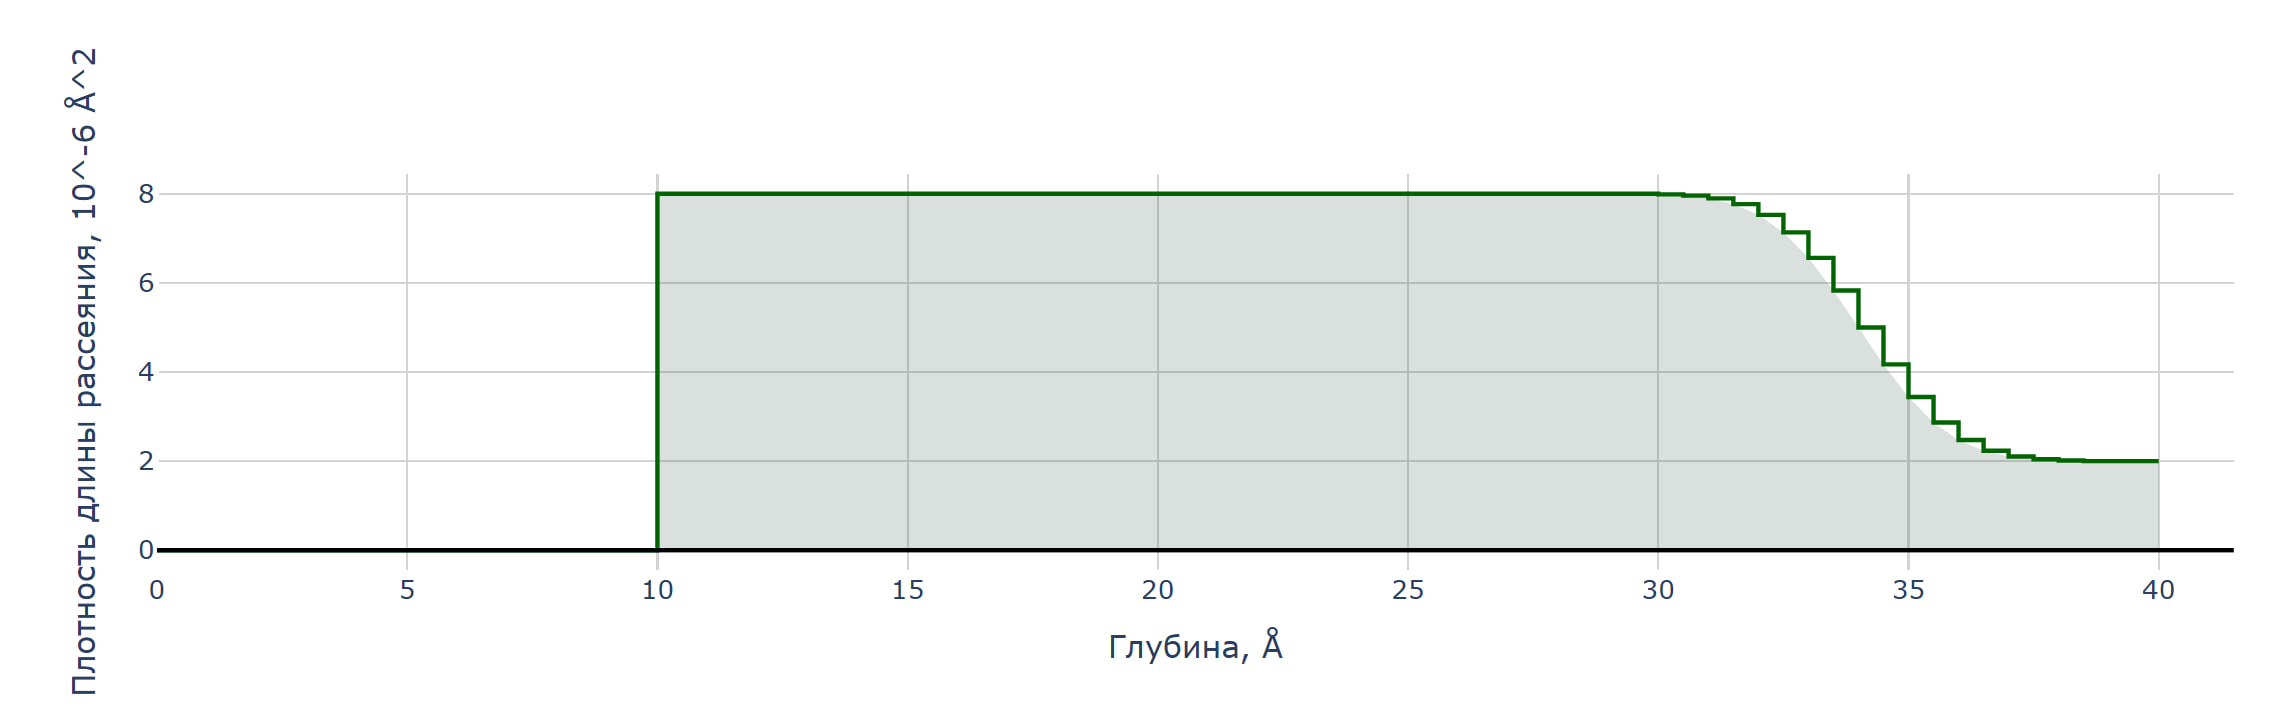
\includegraphics[scale=0.4]{roughness.jpg}
\caption{Модифицированный профиль плотностей длин рассеяния с учётом шероховатости}
\end{figure}

\item \textbf{Динамическая сетка} 

Так как после построения теоретической кривой рефлектометрии к ней будет применена свёртка, необходимо, чтобы для нее было достаточное разрешение: для каждой точки кривой требуется наличие в диапазоне, в котором будет производиться свёртка, того количества точек, которым аппроксимируется гауссов профиль.
С другой стороны, поскольку прямая задача рефлектометрии в последующем будет решаться многократно, требуется ускорить вычисления кривой рефлектометрии. Следовательно, было решено брать минимальное количество точек, необходимое для корректной работы свёртки на моделируемой выборке.
Так, исходя из предположения о локальной гладкости кривой рефлектометрии, можно утверждать, что в диапазоне работы свёртки (зачастую, 11 ближайших точек), шаг сетки остается практически неизменным.
\begin{equation}
    Ndots_{norm}dq_i = 6\sigma q_i,
\end{equation}

где \( \mathrm{Ndots}_{\mathrm{norm}} \) - количество точек, которым аппроксимируется гауссов профиль, 
\( dq_i \) - i-й шаг сетки, 
\( \sigma \) - разрешение установки, 
\( q_i \) - длина волнового вектора на i-й итерации.

Следовательно, получаем рекуррентное соотношение для значений сетки:
\begin{equation}
    q_{i+1} = q_{i} + \frac{6\sigma q_i}{Ndots_{norm}}
\end{equation}

Таким образом, получается минимальный набор точек, необходимый для работы свёртки над моделируемой выборкой измерений.

\section*{Решение обратной задачи}
Основная сложность в задаче рефлектометрии - это решение обратной задачи рассеяния, поскольку она не имеет решения в общем виде.\\
Необходимо подобрать параметры образца так, чтобы данная (экспериментальная) и моделируемая кривые рефлектометрии совпали, или хотя бы были максимально близки друг к другу.
\item \textbf{Функция ошибок}\\
Для оценки "близости" двух кривых была написана функция, называемая функцией ошибок - чем больше несоответствие, тем больше функция ошибок.\\
В стандартных подходах предлагается использовать критерий Пирсона или среднеквадратическое отклонение по каждой точке кривой рефлектометрии. Критерий Пирсона не подходит уже потому, что вес относительного отклонения будет пропорционален значению коэффициента отражения: 
\begin{equation}
    \chi^2 =\sum{\frac{(\Delta R_i)^2}{R_i}}= \sum{R_i(\frac{\Delta R_i}{R_i})^2}
\end{equation}
Среднеквадратическое отклонение по каждой точке кривой рефлектометрии не имеет такой проблемы, однако, обладает другими свойствами, усложняющими решение задачи.\\
При решении задачи рефлектометрии известны параметры образца: плотности длин рассеяния (задаются материалами образца), глубины слоев материалов. Требуется лишь уточнить глубины слоев с учётом шероховатостей. Так, при поиске в реальных диапазонах параметров, кривая рефлектометрии варьируется не сильно. 
Кроме того, график рефлектометрии из себя представляет сложные затухающие колебания, а информацию об их характере несут минимумы и максимумы, то есть экстремумы. Таким образом, точки на кривой рефлектометрии имеют совершенно разную информативность. Так, например, если "колебания" на двух похожих кривых рефлектометрии будут в "противофазе", но с одинаковым характером "колебаний", то функция ошибок будет велика, несмотря на близость параметров к искомым.\\
Так, функция ошибок среднеквадратическое отклонение по каждой точке имеет не только большое количество локальных минимумов, что существенно осложняет поиск минимума, но и весьма трудоёмка с точки зрения счёта - учитываются все точки кривой рефлектометрии.\\
Ввиду вышеперечисленных факторов, было решено написать свою функцию ошибок, наиболее подходящую для задачи рефлектометрии. Так, функция учитывает только информативные точки с одинаковым весом, относительное отклонение для каждой из них не только по оси ординат, но и по оси абсцисс. 
\begin{figure}[H]
\centering
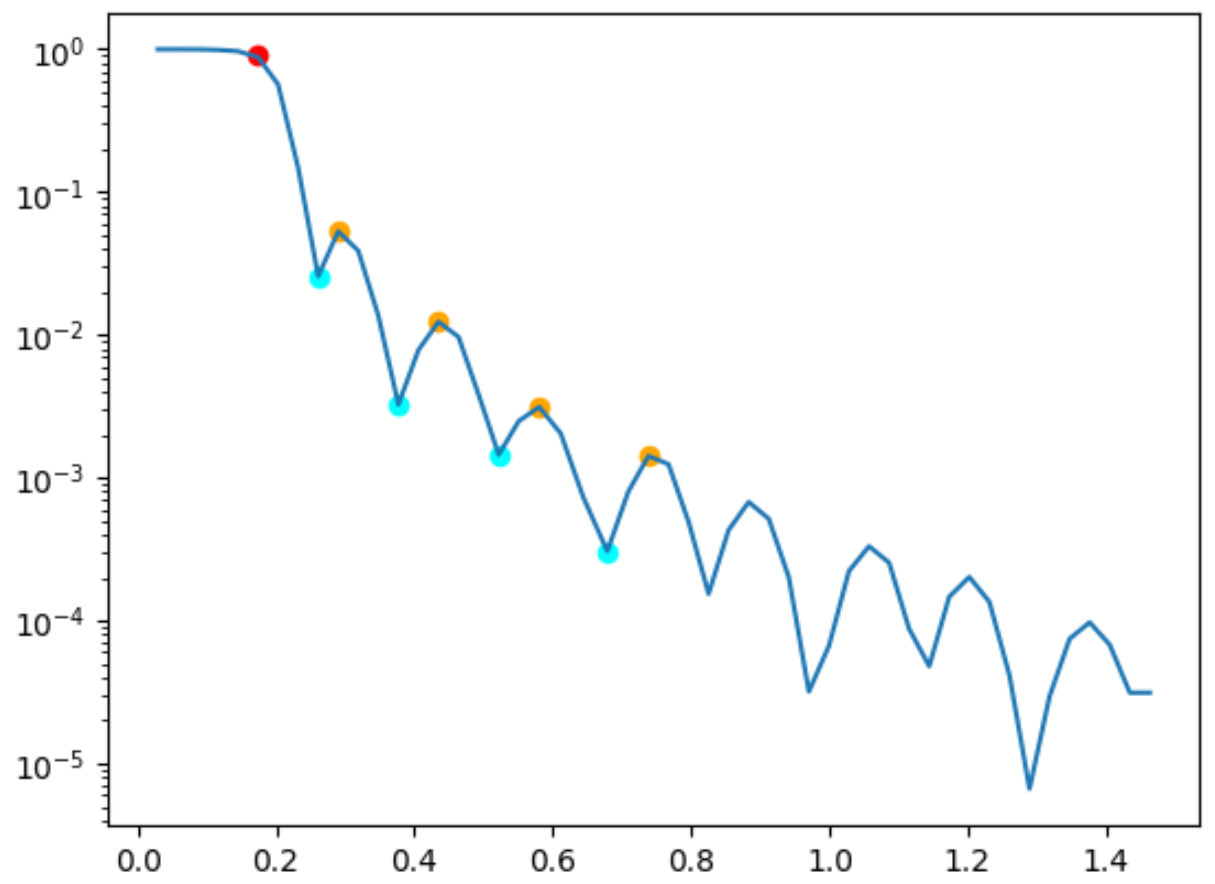
\includegraphics[scale=0.8]{ref_trace.jpg}
\caption{Информативные точки кривой рефлектометрии:\\
критическая точка - красная,\\
первые 4 минимума - голубые,\\
первые 4 максимума - оранжевые.}
\end{figure}


\item \textbf{Поиск минимума функции ошибок} \\
Вышеописанная функция не является строго гладкой и может иметь несколько локальных минимумов, следовательно, наиболее надёжно будут работать стохастические алгоритмы поиска минимума. Однако, такие методы крайне медлительны уже на малых размерностях, а минимум должен быть найден в разумный промежуток времени вне зависимости от числа уточняемых параметров.\\
Следовательно, ввиду относительной гладкости вышеописанной функции, был выбран модифицированный для работы в многомерном кубе алгоритм Бройдена — Флетчера — Гольдфарба — Шанно (L-BFGS-B). Это квазиградиентный метод, что позволяет ему сходиться кратно быстрее, чем стохастическим методам. Градиенты считаются путём численного дифференцирования. 



\end{enumerate}

\subsection*{Полученные данные}

\textbf{Зависимость коэффициента отражения $R(q_z)$} (рис. 8):

На графике наблюдаются осцилляции, характерные для интерференции нейтронных волн в тонких слоях. Период осцилляций соответствует толщине пленки. После свёртки с аппаратной функцией теоретическая кривая демонстрирует сглаживание осцилляций, имитируя влияние ограниченного разрешения установки.

\begin{figure}[H]
\centering
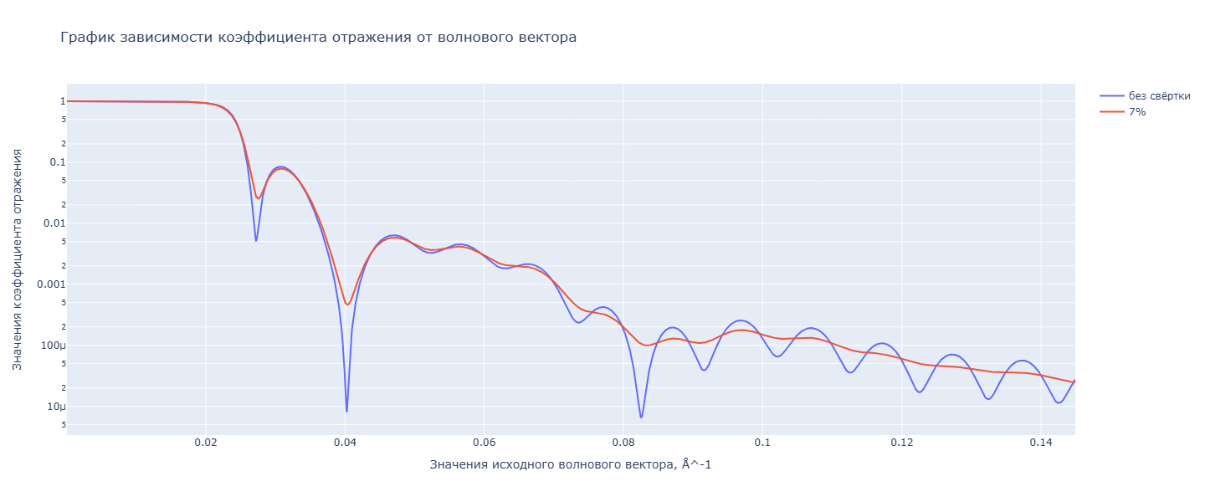
\includegraphics[width=0.9\textwidth]{a0000-img002.png}
\caption{График зависимости коэффициента отражения от волнового вектора}
\end{figure}


\section*{Выводы по разделу}

Исключение спиновой поляризации упростило модель, сохранив её применимость для немагнитных систем. Векторизация матричных операций повысила эффективность вычислений, что особенно важно для анализа многослойных структур. Модель демонстрирует хорошее согласие с экспериментом, подтверждая её работоспособность для задач рефлектометрии на установках с умеренным разрешением.

\printbibliography[title={Список литературы}]

\end{document}